\documentclass[a4j,twocolumn]{jarticle}
\usepackage[utf8]{inputenc}
\usepackage[cmex10]{amsmath}
\usepackage{amssymb,verbatim}
\usepackage[dvipdfmx]{graphicx}
\usepackage{mathrsfs}
\usepackage{here}
\usepackage{tabularx}
\usepackage{listings,jvlisting}
\usepackage{geometry}
\geometry{left=20mm,right=20mm,top=20mm,bottom=20mm}
\fontsize{14pt}{10pt}\selectfont
\def \figref #1{\figurename\ref{#1}}
\def \tbref #1{\tablename\ref{#1}}
\def \equref #1{式(\ref{#1})}
%\vspace{-20cm}
\title{\vspace{-2em}コヒーレント状態を用いた通信の古典通信容量\\
\vspace{0.5cm}
\normalsize{Classical Capacity for Communication with coherent states}}
\date{}
\pagestyle{empty}
\author{量子情報数理研究室\hspace{50mm}米沢将}
\begin{document}
\maketitle
\thispagestyle{empty}
\section{はじめに}
本発表では、コヒーレント状態を用いて通信を行う際の通信容量について調べる。又、増幅器の効果についても評価を行う。

\section{通信路}
通信路に入力される記号$\{a_1,a_2,…,a_r\}$の集合$A_c$を入力アルファベットと呼ぶ。また、通信路から出力される記号$\{b_1,b_2,…,b_r\}$の集合$A_r$を出力アルファベットと呼ぶ。
ここで、$a_i$が入力された時に$b_j$が出力される条件付き確率$P(b_j|a_i)$を要素とする行列を通信路行列と呼ぶ。
定常無記憶通信路の確率的性質は通信路行列
$$T=[p_{ij}],p_{ij}=P(b_j|a_i)$$ $$(i=1,2,\cdots ,q;j=1,2,\cdots,r)$$
で完全に表すことができる。



通信路の例として、2元対称通信路について説明する。
2元対称通信路の通信路行列は以下のようにあらわすことができる。
$$
T=\begin{bmatrix}
1-p&p\\
p&1-p
\end{bmatrix}
(0≦p≦1)$$ 
これを通信路線図を用いて書くと\figref{Fig2_1}のように書くことができる。

    \begin{figure}[H]
        \centering   
        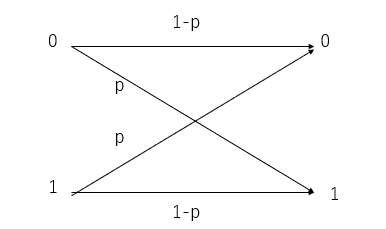
\includegraphics[width=0.4\textwidth]{img/Fig1.png}
        \caption[sample image (png)]{通信路線図}
        \label{Fig2_1}
    \end{figure}


ここで、$0$が入力されると確率 $1-p$で$0$が出力され、確率$p$で$1$が出力されることがわかる。
一方$1$が入力されると確率$p$で$0$が出力され、確率1-pで$1$が出力される。

\section{エントロピーと通信容量}
通信容量は、通信路で伝達できる最大の($1$記号当りの)情報量のことである。
通信容量$C$は次式によって与えられることが知られている。
$$
C=\max_{P_X}I(X;Y)  (1)
$$
ここで、$\max_{P_X}$は先験確率$P_X$を動かして最大値を求めることを意味している。
すなわち通信容量は相互情報量I(X;Y)を$P_X$で最大化したものとなっている。相互情報量は、出力$Y$を知ったときに得る$X$に関する情報量のことで、通信路で伝達される情報量を表している。



相互情報量について詳しく見るために、エントロピーについて説明をする。
エントロピーとはXに関する曖昧さを表す量で、
$$
H(X)=-\sum_xP_X(x)\log P_X(x)
$$
によって求めることができる。
条件付きエントロピーは、
$Y$の値を知った時に$x$に関して残る平均の曖昧さを表す量で、
次式によって計算することができる。
$$
H(X|Y)=\sum_xP_Y(y)H(X|Y=y)$$
$$
H(X|Y=y)=-\sum_xP(x|y)\log P(X|Y)
$$




これらの式を用いて相互情報量は
$$
I(X;Y)=H(X)-H(X|Y)
$$
と定義される。エントロピー$H(X)$は、Xに関する曖昧さを表しており、
条件付きエントロピー$H(X|Y)$は、$Y$の値を知った時に$x$に関して残る平均の曖昧さ
を表している。したがって$H(X)$から$H(X|Y)$を引くとYの値を知ることにより、消えた$X$の曖昧さになる。
すなわち相互情報量は、出力$Y$を知ったときに得る$X$に関する情報量となっている。
\figref{Fig3_1}は相互情報量とエントロピーの関係を表している。


    \begin{figure}[H]
        \centering   
        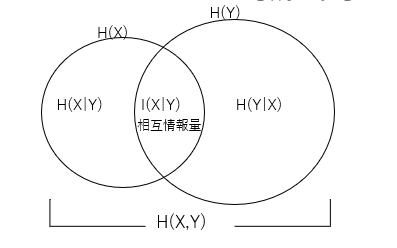
\includegraphics[width=0.5\textwidth]{img/Fig2.png}
        \caption[sample image (png)]{相互情報量とエントロピーの関係}
        \label{Fig3_1}
    \end{figure}


$H(X)$から$H(X|Y)$を引くと相互情報量$I(X|Y)$となるが、
$H(Y)$から$H(Y|X)$を引いても相互情報量$I(X|Y)$が得られることが知られている。


次に2元対称通信路の通信容量について計算する。
式(1)において、最適な$P_X$は、$P_X(0)=P_X(1)=1/2$となることが知られているので、
この事実を使って通信容量を計算する。
$$
C=p\log_2p-(1-p)\log_2(1-p)
$$

\section{コヒーレント状態を用いた通信}
複素振幅αを持つ光の状態をコヒーレント状態と呼ぶ。コヒーレント状態$|\alpha\rangle$は以下のような式で与えることができる。

\begin{equation}
|\alpha\rangle=\sum_nC_n|n\rangle 
C_n=
\end{equation}


ここでは、$\alpha$を実数として、コヒーレント状態 $|\alpha\rangle$、$|-\alpha\rangle$を用いて通信について考える。

この通信では、$0$に対して$|-\alpha\rangle$を、$1$に対して$|\alpha\rangle$を送信する。
受信者はホモダイン測定を行い、その測定値に対してしきい値処理をおこなって$0$または$1$出力する。ホモダイン測定では、コヒーレント状態の複素振幅$\alpha=x+iy$の$x$成分を測定する。

    \begin{figure}[H]
        \centering   
        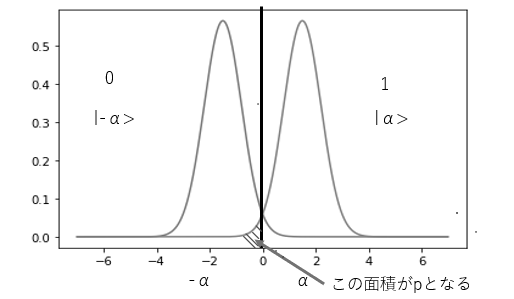
\includegraphics[width=0.5\textwidth]{img/Fig3.png}
        \caption[sample image (png)]{コヒーレント状態をホモダイン測定した場合の出力の確率分布}
        \label{Fig4_1}
    \end{figure}




\figref{Fig4_1}は、コヒーレント状態$\alpha$と$-\alpha$の測定値の確率分布のグラフを表している。この分布はそれぞれ分散$1/4$の正規分布となっている。
そして、閾値を$0$に設定し測定値が$0$より小さい場合は$0$、大きい場合は$1$を受信したと判断する。
したがって、この通信路は2元対称通信路となり、この面積が誤り確率$p$を表している。
したがって、この面積を計算すると通信容量を求めることが可能になる。


誤り確率$p$は、以下のような積分によって計算することができる。
$$
\int_{-\infty}^{x_0}f(x)dx
$$この積分は累積分布関数を用いて計算することができる。
累積分布関数はPythonを用いると以下のように書くことによって計算することができる。

\begin{lstlisting}[caption=累積分布関数]
p=norm.cdf(0,loc=x,scale=0.25)
\end{lstlisting}

また、通信容量は以下のように書いて計算することができる。

\begin{lstlisting}[caption=通信容量]
C=1+p*np.log(p)+(1-p)*np.log(1-p)
\end{lstlisting}


    \begin{figure}[H]
        \centering   
        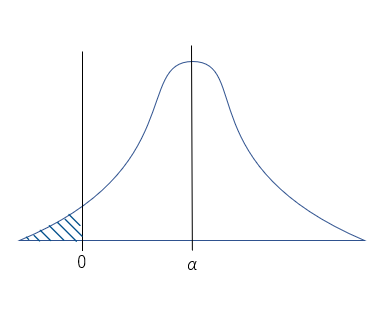
\includegraphics[width=0.5\textwidth]{img/Fig4.png}
         \caption[sample image (png)]{正規分布}
        \label{Fig4_2}
    \end{figure}

\figref{Fig4_2}はコヒーレント状態$|x\rangle$の測定値の確率分布のグラフをわかりやすくしたものである。


\begin{lstlisting}[caption=αの変化で変わる通信容量]
x=np.arange(0,5,0.01)
p=norm.cdf(0,loc=x,scale=0.25)
c=1+p*np.log(p)+(1-p)*np.log(1-p)
plt.plot(x,c)
\end{lstlisting}
\figref{Fig4_3}は、通信容量の計算の結果である。
信号$\alpha$と$-\alpha$を区別することが容易となるので誤り率$p$はほとんど$0$となる。
そのため\figref{Fig4_3}において、$\alpha$の値が大きくなると、通信容量$1$に近づいている。

  \begin{figure}[H]     
  \centering   
  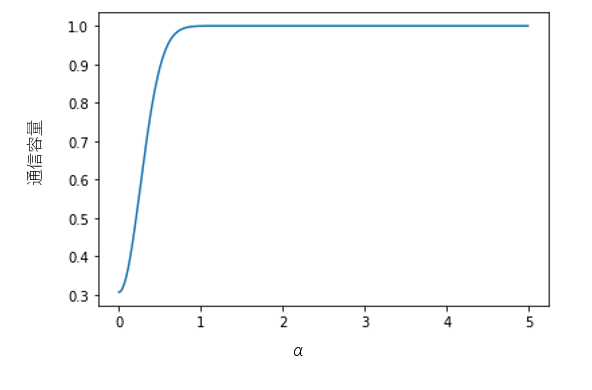
\includegraphics[width=0.5\textwidth]{img/Fig5.png}
\caption[sample image (png)]{$\alpha$の変化で変わる通信容量}     \label{Fig4_3}
\end{figure}

減衰通信路を用いた通信を行う場合の通信容量を計算する。
以下は通信容量のグラフを書くためのプログラムである。
\begin{lstlisting}[caption=減衰通信路の通信容量,label=program5_1]
import japanize_matplotlib
x=np.arange(0,5,0.01)
y1=[]
arate=0.05 #@param {type: "number"}
for x_val in x:
  q_state=Qstate(x_val)
  q_state.attenuate(arate)
  p=norm.cdf(0,loc=q_state.alpha,scale=np.sqrt(q_state.a[0][0]))
  c=1+p*np.log(p)+(1-p)*np.log(1-p)
  y1.append(c)
y2=[]
for x_val in x:
  q_state=Qstate(x_val)
  q_state.attenuate(np.sqrt(arate))
  q_state.amplificate(1/np.sqrt(arate))
  q_state.attenuate(np.sqrt(arate))
  p=norm.cdf(0,loc=q_state.alpha,scale=np.sqrt(q_state.a[0][0]))
  c=1+p*np.log(p)+(1-p)*np.log(1-p)
  y2.append(c)

plt.plot(x,y1,label="増幅器なし",c="black",ls="dotted")
plt.plot(x,y2,label="増幅器あり",c="black",ls="-")
plt.legend()
plt.show()
\end{lstlisting}

\figref{Fig5_1}は、透過率$\lambda=0.05$の時の通信容量のグラフを表している。実線は増幅器ありの場合、点線は増幅器なしの場合のグラフである。グラフの横軸は信号の振幅値を表し、縦軸は通信容量を表している。グラフより、透過率$\lambda=0.05$の場合は、増幅器を設置することにより、通信容量を大きくする効果があることがわかる。

    \begin{figure}[H]
        \centering   
        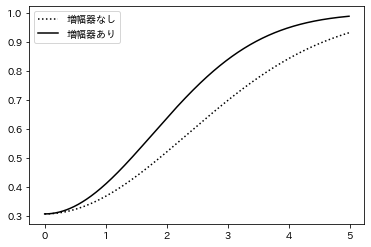
\includegraphics[width=0.5\textwidth]{img/Fig5_1.png}
        \caption[sample image (png)]{$\lambda=0.05$のときの通信容量の変化}
        \label{Fig5_1}
    \end{figure}

\newpage
\figref{Fig5_2}は、透過率$\lambda=0.1$の時の通信容量のグラフを表している。実線は増幅器ありの場合、点線は増幅器なしの場合のグラフである。グラフの横軸は信号の振幅値を表し、縦軸は通信容量を表している。グラフより、透過率$\lambda=0.1$の場合は、増幅器を設置することにより、通信容量は大きいが、$\lambda=0.05$の時よりほどではないことがわかる。

    \begin{figure}[H]
        \centering   
        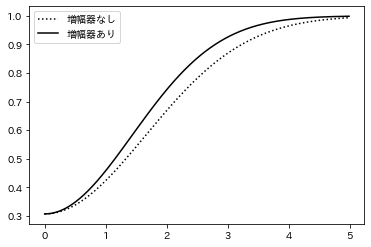
\includegraphics[width=0.5\textwidth]{img/Fig5_2.png}
        \caption[sample image (png)]{$\lambda=0.1$のときの通信容量の変化}
        \label{Fig5_2}
    \end{figure}



\section{まとめ}
今回の研究で、減衰通信路を用いた通信を行った。その結果、透過率を上げていくにつれ、増幅器を使用しても通信容量がほぼ変化しない部分があることに気づいた。また、透過率をそれ以上上げても通信容量がほぼ変化しないことにも気づいた。


\begin{thebibliography}{9}
\bibitem{Futami}Fumio Futami and Osamu Hirota,Two Months Field
Transmission Test of 2.5-Gb/s Y-00 Cipher in 160-km (40 km x 4
spans)Installed Optical Fiber Cable for Secure Optical Fiber Communications,Tamagawa University Quantum ICT Research Institute Bulletin, Vol.2, No.1, 15-17, 2012 

\bibitem{久保}久保貴星,光通信量子暗号のシミュレーション, 玉川大学工学部情報通信工学科卒業論文, 2020 
\end{thebibliography}
\end{document}
